\documentclass{trkut}% Reaalkooli vormistus. Muidu "report" või "article".
\usepackage[style=trkut]{biblatex}% Kasutatud kirjanduse genereerimine
\usepackage{pgfplots}
\usepackage{amsmath}
\usepackage{siunitx}
\usepackage{wasysym}
\usepackage{verbatim}
\usepackage{listings}
\addbibresource{viited_eesnimi_perekonnanimi.bib}% Viidete info fail
\defbibheading{bibliography}{\addchap{#1}}% Lisame kasutatud materjalid sisukorda

\pealkiri{Atmosfääri mudeldamine ja katseandmete põhjal täpseima mudeli leidmine} % Kahel real
\autor{Jarl Patrick Paide}
\klass{11.a}
\juhendaja{õp Mart Kuurme }

\begin{document}
\maketitle% Tiitelleht
\tableofcontents% Sisukord

\addchap{Sissejuhatus}
\nummerdame% See käsk peab olema kohe peale sissejuhatust
%See teema on aktuaalne, kuna see on väga huvitav ja ma tahan seda uurida...
Globaliseeruvas ja ülerahvastatud maailmas on Maa atmosfääri reostatus üks kõige olulisemaid probleeme. Atmosfääri reostusega kaasneb kasvuhooneefekt - kliima soojenemine, mis omakorda viib maailmamere tõusule. Atmosfääri mudeldamine aitab mõista atmosfääris toimuvaid protsesse ja leida lahendusi atmosfääri seisundi parandamiseks. Mudeli andmeid saab kasutada globaalse atmosfääri mudeli väljatöötamisel.

Uurimistöö eesmärk on leida vaatlusandmete alusel võimalikult täpne mudel, mis kirjeldaks atmosfääri temperatuuri ja rõhu seoseid vastavalt kõrgusele maapinnast. Uurimisküsimus on "Millised seosed on atmosfääris mõõdetavate parameetrite vahel - temperatuur, rõhk ja kõrgus maapinnast?".

Uurimistöö hüpotees on, et atmosfääri madalamates kihtides toimuvad termodünaamilised protsessid on adiabaatilised protsessid.

Uurimistöö alguses leitakse eeldusel, et atmosfääris toimuvad termodünaamilised protsessid on adiabaatilised protsessid, seosed temperatuuri, rõhu ja kõrguse vahel.

Praktilises osas tehakse mõõtmisi heeliumõhupalli külge kinnitatud mõõteriistaga, mis lennutatakse stratosfäärini ja pärast kontrollitakse katseandmete põhjal teoreetilises osas saadud seoste kehtivust.

Uurimistöö autor soovib tänada kõiki katse korraldamisel ja läbiviimisel aidanud inimsei ning uurimistöö juhendajat, kes andis head nõu uurimistöö teostamisel.





\chapter{Mudeli teooreetilised alused}
Käesolevas osas leitakse seosed, kuidas kirjeldada atmosfääris rõhu ja temperatuuri sõltuvust kõrgusest.

Atmosfääris tekib rõhk kõrgemal olevate õhukihtide raskusjõu poolt tekkinud jõust. Kuna kõrguse kasvades vähneb kõrgemal asuva õhu mass, siis väheneb ka rõhk kõrguse kasvades. Rõhu erinevus erinevatel kõrgustel toob kaasa rõhkude vahest tingitud ülespoole suunatud jõu, mida tasakaalustab gravitatsioonijõud. Rõhk muutub $dp$ võrra kõrguse $dz$ võrra kasvades, kui õhu tihedus kõrgusel $z$ on $\rho$, järgnevalt \parencite[67--68]{raamat1}:
\begin{equation}\label{eq10}
dp=-\rho gdz.   
\end{equation}

On olemas erinevaid gaasi mudeleid. Nendest kõige tuntum on ideaalse gaasi olekuvõrrand. Ideaalne gaas erineb reaalsest gaasist kahe eelduse poolest. Ideaalses gaasis ei arvestata osakestevahelisi vastastikjõude ja ideaalses gaasis lihtsustatakse, et osakestel on tühiselt väike suurus. Võib eeldada, et gaas on ideaalne siis, kui rõhk on väike võrreldes kriitilise rõhuga ja temperatuur on kõrge võrreldes kriitilise temperatuuriga. Kui rõhk on kõrge, siis on osakestevahelisi kokkupõrkeid palju ja osakeste suurus saab oluliseks. Kui temperatuur on madal, siis liiguvad osakesed aeglaselt ja osakestel on rohkem aega olla üksteise mõjuväljas ja saada mõjutatud. Kui vaadata atmosfääri, siis kõige kõrgem rõhk on Maa lähedal ja kõrguse suurenedes see väheneb, millega väheneb ka osakestevaheline vastasmõju. Atmosfääris olevad rõhud on väikesed, võrreldes õhu kriitilise rõhuga. Temperatuur võib langeda atmosfääris küll madalale, aga mitte piisavalt madalale, et see läheneks kriitilisele temperatuurile. Seega võib eeldada, et atmosfääris olevad gaasid käituvad kui ideaalsed gaasid. Ideaalse gaasi olekuvõrrand on:
\begin{equation}\label{eq8}
pV=\nu RT ,
\end{equation}
kus $p$ on gaasi rõhk, $V$ on gaasi ruumala, $\nu = \frac{m}{\mu}$ on gaasi kogus moolides, kus $m$ on gaasi mass ja $\mu$ on gaasi molaarmass, $R$ on universaalne gaasikonstant ja $T$ on gaasi temperatuur \parencite{IGasKhan}.


Kuna selle uurimistöö käigus koguti katseandmeid troposfääris ja stratosfääris, uuritakse ainult neid piirkondi. Joonisel \ref{profile} on näha, kuidas temperatuur muutub kõrguse kasvades. Stratopausis on üks temperatuuri maksimume. Seal olev kõrge temperatuur on otse tingitud UV kiirguse neeldumisest osoonikihis. Kuigi osooni kiht on kõige tihedam madalamal stratosfääris umbes \SI{20}{km} ja \SI{30}{km} vahel, on temperatuur ikkagi kõige kõrgem umbes \SI{50}{km} juures. See on tingitud osooni kihi läbipaistmatusest UV kiirguse jaoks, mistõttu suurem osa kiirgusest neeldub kõrgemal. Troposfäär ei ole mõjutatud Päikese kiirgusest, kuna see on läbipaistev. Erinevalt stratosfäärist ringleb õhk troposfääris palju. Troposfääri soojendab maapind, mida soojendab Päike. Soojalt maapinnalt tõustes hakkab rõhk vähenema ja ideaalse gaasi olekuvõrrandi kohaselt hakkab temparatuur langema \parencite[25--26]{book:779878}.

\begin{figure}[h]
	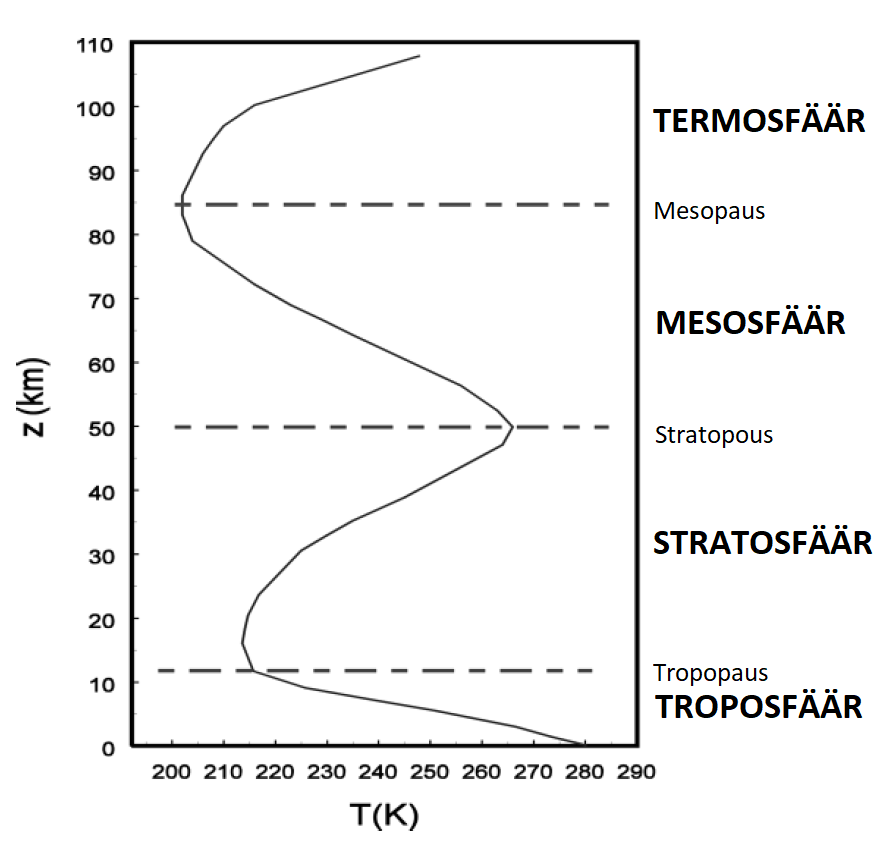
\includegraphics[width=0.5\textwidth]{PicGra/Profile2.png}
	\caption{Temperatuuri sõltuvus kõrgusest}
	\allikas{\cite{book:779878}}
	\label{profile}% Selle järgi viidatakse, see rida peab olema pärast \caption
\end{figure}

Tropsfääris on õhk pidevas liikumises. Ning kuna troposfääris soojeneb õhk ainult maapinna lähedal, siis võib oletada, et termodünaamilised protsessid, mis toimuvad õhu üles ja alla liikumisest, mille käigus muutub õhu rõhk, on adiabaatilised protsessid, ehk õhu vahel soojusvahetust ei toimu.


\section{Adiabaatiline protsess}
Termodünaamika esimene seadus on
\begin{equation}\label{eq1}
dU = dQ - dA ,
\end{equation}
kus $dU$ on gaasi siseenergia muutus, $dQ$ on soojushulk ja $dA$ on töö. Gaasi siseenergia $U$ avaldub vabadusastmete $i$ kaudu järgneva seose abil:
\begin{equation}\label{eq5}
U = \frac{i}{2} \nu R T.
\end{equation}
Konstantse ruumala puhul tööd ei tehta, seega kogu soojus läheb siseenergia suurendamiseks. Saame soojusmahutavuse, võttes siseenergia muudust tuletise temeratuuri järgi:
\begin{equation}\label{eq6}
C_V = \frac{dQ}{dT}=\frac{i}{2}\nu R .
\end{equation}
Molaarset soojusmahutavust saab avaldada valemiga $c_V = \frac{C_V}{\nu}$, saades molaarseks soojusmahutavuseks
\begin{equation}\label{eq7}
c_V = \frac{i}{2}R .
\end{equation}
Kui aga vaadata isobaarilist protsessi, siis olekuvõrrandist tuleneb: $pdV=\nu RdT$, ning gaas teeb tööd $dA = pdV = \nu RdT$. Avaldades need valemisse \ref{eq1} saadakse:
\begin{equation*}
dQ = dU + dA = \frac{i+2}{2} \nu R dT ,
\end{equation*}
millest järeldub:
\begin{equation*}
c_p=\frac{i+2}{2}R.
\end{equation*}
Samuti saab näidata $c_V$ ja $c_p$ vahelist seost:
\begin{equation}\label{eq9}
c_p =\frac{i+2}{2}R = \frac{i}{2}R + R = c_V + R.
\end{equation}
Adiabaatiline protsess on termodünaamiline protsess, mille käigus ei toimu soojusvahetust väliskeskkonnaga, seega valemis \ref{eq1} $dQ=0$. Gaasi poolt tehtud töö on $d A=pdV$ ja gaasi siseenergia muut on $dU=\nu c_VdT$. Sellest järeldub:
\begin{equation}\label{eq2}
\nu c_VdT = -pdV.
\end{equation}
Ideaalse gaasi olekuvõrrandist \ref{eq8} saadakse tuletist võttes ja $dT$ avaldades järgneva seose:
\begin{equation}\label{eq3}
dT = \frac{pdV+Vdp}{\nu R}.
\end{equation}
Asendades valemi \ref{eq3} valemisse \ref{eq2} saadakse uus seos:
\begin{equation}\label{eq4}
pdV(c_V+R)+c_VVdp=0.
\end{equation}
Asendades siia sisse valemi \ref{eq9} ja adiabaadi näitaja $ \gamma \equiv \frac{c_p}{c_V}$ saadakse võrrand
\begin{equation*}
\gamma \frac{dV}{V} + \frac{dp}{p} = 0.
\end{equation*}
Seda integreerides saadakse uus võrdus:
\begin{equation*}
 \int \gamma \frac{dV}{V} + \frac{dp}{p} = \gamma \ln(V) + \ln(p) = Const.
\end{equation*}
Sellest saab järeldada
\begin{equation*}
pV^\gamma = Const.
\end{equation*}
Samuti, kasutades ideaalse gaasi olekuvõrrandit, saab tuletada järgneva seose:
\begin{equation}\label{eq13}
p^{1-\gamma}T^\gamma = Const.
\end{equation}
Seega, kui vaadata mingit kogust gaasi adiabaatilises protsessis, siis jääb antud võrduse väärtus gaasi parameetrite muutumisel samaks \parencite{JKtermo}.

\section{Adiabaatiline temperatuurigradient }
Selles osas tuletatakse temperatuuri gradient adiabaatilise protsesi puhul. Valemist \ref{eq13} saadakse
\begin{equation*}
d\ln(p^{1-\gamma}T^\gamma) = 0,
\end{equation*}
millest saadakse
\begin{equation}\label{eq17}
\frac{dp}{p} = \frac{\gamma}{\gamma-1}\frac{dT}{T}.
\end{equation}
Asendades seosed \ref{eq10} ja \ref{eq8} seosesse \ref{eq17} saadakse temperatuurigradient:
\begin{equation}\label{eq11}
\Gamma \equiv \frac{dT}{dz}=-\frac{\gamma-1}{\gamma} \frac{\mu g}{R} = -\frac{R}{c_p}\frac{\mu g}{R} = -\frac{\mu g}{c_p}.
\end{equation}
Valem \ref{eq11} kehtib juhul, kui õhus pole veeauru. Kui õhus on küllastumata veeaur, toimuvad atmosfääris ikkagi adiabaatilised protsessid. Sellisel juhul kehtib valem 
\begin{equation*}
\Gamma = -\frac{g}{c_m} ,
\end{equation*}
kus $c_m$ niiske õhu erisoojus. Erisoojus avaldub molaarsest erisoojusest kujul $c_m=\frac{c_p}{\mu}$. Kui asendada nüüd valemisse õhu erisoojuse osakaalud, saadakse lõplikuks valemiks
\begin{equation}\label{eq12}
\Gamma = -\frac{g}{(1-\omega)c_{o} + \omega c_{v}} ,
\end{equation}
kus $c_{o}$ on õhu erisoojus, $c_{v}$ on vee auru erisoojus ja $\omega$ on vee massiosakaal \parencite[36]{raamat2}.

\section{Rõhu muutus kõrgusega }
Integreerides valemit \ref{eq11} saadakse
\begin{equation*}
\int_{T_0}^{T} dT = \int_{0}^{z} \Gamma dz
\end{equation*}
\begin{equation*}
T-T_0 = \Gamma z,
\end{equation*}
kus $T_0$ on temperatuur algpunktis ja $T$ on temperatuur kõrgusel $z$ algpunktist. Avaldist teisendades saadakse:
\begin{equation*}
T = T_0 \left(1+\frac{\Gamma}{T_0}z\right).
\end{equation*}
Kasutades nüüd seost \ref{eq13}, saab eelmise valemi ümber kirjutada kujul:
\begin{equation*}
p=p_0 \left(1+\frac{\Gamma}{T_0}z\right)^{\frac{\gamma}{\gamma-1}}.
\end{equation*}
Astendaja saab asendada kujuga
\begin{equation*}
\frac{\gamma}{\gamma-1} = \frac{c_p}{R} = -\frac{g\mu}{\Gamma R},
\end{equation*}
saades lõplikuks valemiks:
\begin{equation}\label{eq15}
p=p_0 \left(1+\frac{\Gamma}{T_0}z\right)^{ -\frac{g\mu}{\Gamma R}}.
\end{equation}
Seega, kui on teada algpunktis olev rõhk $p_0$, temperatuur $T_0$ ja temperatuurigradient $\Gamma$, on võimalik leida seda valemit kasutades rõhk kõrgusel $z$ algpunktist \parencite{Texas}.



\section{Veeauru kondenseerumine}
Kui niiske õhk tõuseb kõrgemale, siis langeb temperatuur ja rõhk. Kui õhk jahtub ja rõhk väheneb, siis väheneb ka õhu võime hoida vett auruna endas ja veeaur kondenseerub väga väikesteks tilkadeks. Veeaurul on lihtsam kondenseeruda, kui veeaur saab kondenseeruda osakese külge. Nendeks osakesteks on tavaliselt tolm või õietolm. Kui piisavalt palju veeauru kondenseerub väikeste osakeste külge, siis moodustub pilv \parencite{raamat1}.

Vee kondenseerumisel pilvedes eraldub soojus, seega pilvedes toimuv termodünaamiline protsess ei vasta adiabaatilisele protsessile. Kuid kuna väljaspool pilvi veeaur ei kondenseeru, siis pilvedest madalamal ja kõrgemal termodünaamilised protsessid on adiabaatilised protsessid.

Järgnevalt leitakse suhe õhust välja aurustunud vee ja õhu masside vahel. Temperatuuri gradient vahetult pilve all on $\Gamma$, temperatuur pilve all on $T_0$, temperatuur pilvede kohal $z$ võrra kõrgemal algtemperatuurist on $T_2$, vaadeldava õhu mass on $m_a$ ja sellest õhust kondenseerunud õhu vee mass on $m_v$. Kui pilvi ei oleks, siis muutuks temperatuur edasi vastavalt temperatuurigradiendile. Seega temperatuur oleks $T_2$ asemel
\begin{equation*}
T_1 = T_0 + \Gamma z.
\end{equation*}
Veearu annab kondenseerumisel ära energia
\begin{equation*}
\Delta U = L m_v
\end{equation*}
kus $L$ on aurustumissoojus. See energia läheb õhu siseenergia suurendamiseks. Gaasi siseenergiat saab arvutada valemiga \ref{eq5}, seega siseenergia muut on
\begin{equation*}
\Delta U =\frac{i}{2}\frac{m_a}{\mu}RT_2 - \frac{i}{2}\frac{m_a}{\mu}RT_1  = \frac{i}{2}\frac{m_a}{\mu}R\left(T_2 - T_0 - \Gamma z\right).
\end{equation*}
Seega saab avaldada masside suhte järgnevalt:
\begin{equation*}
\frac{m_v}{m_a} = \frac{i}{2}\frac{R}{\mu L}\left(T_2- T_0 - \Gamma z\right).
\end{equation*}



\section{UV kiirgus stratosfääris}
Troposfäärist kõrgemal asub stratosfäär. Kuna UV kiirguse neeldumisel eralduv soojus antakse õhule juurde, siis pole tegu enam adiabaatilise protsessiga. Järgnevalt võrreldakse olukorda, kus UV kiirgus ei neeldu stratosfääris, tegeliku olukorraga, kus UV kiirgus neeldub stratosfääris. Arvutatakse gaasi siseenergiate suhe nendes erinevates olukordades. Temperatuur stratosfääri ja troposfääri vahelisel alal on $T_0$ ja temperatuurigradient samal kõrgusel on $\Gamma$. Temperatuur $z$ võrra kõrgemal stratosfääris on $T_2$. Kui UV kiirgus ei neelduks, siis temperatuur langeks edasi temperatuurigradiendi järgi. Sellisel juhul oleks temperatuur $z$ võrra kõrgemal algpunktist
\begin{equation*}
T_1 = T_0 + \Gamma z.
\end{equation*}
Siseenergia avaldub kujul:
\begin{equation*}
U = \frac{i}{2}\gamma RT.
\end{equation*}
Seega on siseenergia 
\begin{equation*}
\frac{U_2}{U_1} = \frac{\frac{i}{2}\gamma RT_2}{\frac{i}{2}\gamma R\left(T_0 + \Gamma z\right)} = \frac{T_2}{T_0+\Gamma z}
\end{equation*}
korda suurem siis, kui UV kiirgus neeldub, võrreldes olukorraga, kui UV kiirgust ei neeldu.


\chapter{Katse ülesehitus}
Katse käigus mõõdeti atmosfääris, troposfääris ja stratosfääri madalamates kihtides rõhku, temperatuuri ja õhuniiskust. Selle jaoks kasutati heeliumõhupalli külge kinnitatud sondi, mis tegi mõõtmisi. Andmeid koguti heeliumiga täidetud õhupalliga kaasa saadetud sondiga, mis mõõtis erinevaid andmeid.

Põhilisteks andmeteks on kõrgus, asukoht, aeg, välistemperatuur ja rõhk. Sondi pardal oli Raspberry Pi arvuti. Õhupall kerkis atmosfääri kõrgematesse kihtidesse, sest üleslükkejõud ületab kerge gaasi ja sondi massi poolt tekitatud raskusjõu. Kõrgemale tõustes rõhk väheneb. Et õhupalli siserõhk oleks tasakaalus välisrõhuga, suureneb õhupalli ruumala, kuni õhupall lõhkeb ülepingest. Peale seda kukub sond alla ja leitakse GPS jälgija abiga üles.


\section{Katse eesmärk}
Katsel oli kaks eesmärki. Üks eesmärk oli käesoleva uurimistöö jaoks koguda atmosfäärist andmeid, et testida reaalsete katseandmete kokkulangemist teoreetiliselt tuletatud valemitega. Teiseks tekkis idee tuua midagi atmosfäärist kaasa ja see idee suunati edasi Reaalkooli põhikooli õpilastele, kes arendasid ideed edasi ja otsustasid stratosfäärist õhku läbi filtri juhtida ja sellega koguda stratosfäärist tolmu ja muid suuremaid osakesi. Tolmu kogumine ei käi selle uurimistöö juurde.

Esimeses peatükis koostatud mudeli kontrollimiseks oli vaja koguda atmosfääri erinevate kõrguste andmeid temperatuuri, rõhu ja õhuniiskuse kohta.

\section{Katsemetoodika valik}
Selles uurimistöös tehtud katsed on tehtud koostöös Eesti kosmosekoolide võrgustikuga (kosmosekoolid.ee), mille asutaja Väätsa põhikool oli enne selle uurimistööga tehtud lendu teinud kaks lendu. Esimene lend, mis tehti 29. märtsil 2018, kestis umbes kaks tundi, kus kõrgeim punkt, milleni jõuti, oli \SI{26474}{m}. Sellele kõrgusele jõuti pooleteise tunniga. Kokku tehti 220 mõõtmist. Mõõdeti kellaaega, laiuskraadi, pikkuskraadi, kõrgust, kapsli sisetemperatuuri, välistemperatuuri ja rõhku. Teine lend tehti 11. mail 2018 ning seekord kestis lend peaaegu neli tundi. Kolme ja poole tunniga jõudis sond kõrgusele \SI{32608}{m}. Katse tegijad vähendasid teisel lennul õhupallis heeliumi kogust, mille tõttu oli tõusmise kiirus väiksem, aga õhupall lõhkes hiljem ja jõuti kõrgemale. Teisel lennul tehti 4300 mõõtmist ja mõõdeti samu parameetreid.

Katse korraldamiseks ja läbiviimiseks vajalikud oskused saadi Eesti kosmosekoolide võrgustiku poolt korraldatavalt koolituselt ja sealt on pärit ka vastav metoodika, kuidas katselendu läbi viia.

\section{Katse planeerimine}
Alguses oli plaanis heeliumpall lendu lasta Väätsa staadionilt, aga kasutades Internetis olevat kalkulaatorit leheküljel http://predict.habhub.org/, oli ennustusest näha, et sond oleks kukkunud Jõhvi lähedale. Kuna eksimusruum võib olla suur ning Venemaa piir ja meri ei olnud kukkumiskohast kaugel, siis otsustati lennu start teha võimalikult edelast nii, et edelatuultega kalduks sond Kesk-Eestisse. Rihtides lõppsihtkohta Paide peale, otsustati start teha Varblast Pärnumaalt.

Lennu jaoks oli vajalik saada Lennuametilt kooskõlastus. Selle jaoks kirjutati nädal aega enne planeeritud lendu ja küsiti kooskõlastust asukoha järgi. Kuna viimasel hetkel stardi asukoht muutus, pidi uue kooskõlastuse küsima, aga see ei olnud probleem. Vahetult enne lendu pidi telefoni teel saama viimase kinnituse stardiks.

Sondi ehitamise eest võttis vastutuse enda peale Tallinna Reaalkooli põhikooli õpilaste robootikameeskond Viirus. Sondi põhiehitusmaterjaliks oli penoplast ja puidust tikud. Sond pidi hoidma sisetemperatuuri madalate välistemperatuuride eest, et sisemuses olev elektroonika töötaks. Samuti pidi korpus vastu pidama kukkumisele ning sondi korpus pidi olema võimalikult kerge. Selle tõttu valiti korpuse materjaliks penoplast ja tikud. Sondi sees olev ruum oli jaotatud kaheks. Sondi sisemus on näidatud joonisel \ref{sond1}, kus vasakul on sondi alumine osa ja paremal on ülemine osa. Alumises olid kaks toru, mis olid paralleelsed ja läbisid sondi kere. Nende sees olid klapid, ventilaator ja filtrid. Ülemises osas oli kogu tehnika. Mõõtmisi tegi ja klappe avas Raspberry Pi arvuti. Voolu andis nii ventilaatoritele kui ka Raspberry Pi'le akupank. Raspberry Pi külge oli kinnitatud raadioantenn, GPS-antenn, mootor klappide jaoks ja andur BME280, mis mõõtis õhurõhku, temperatuuri ja õhuniiskust.
\begin{figure}[h]
	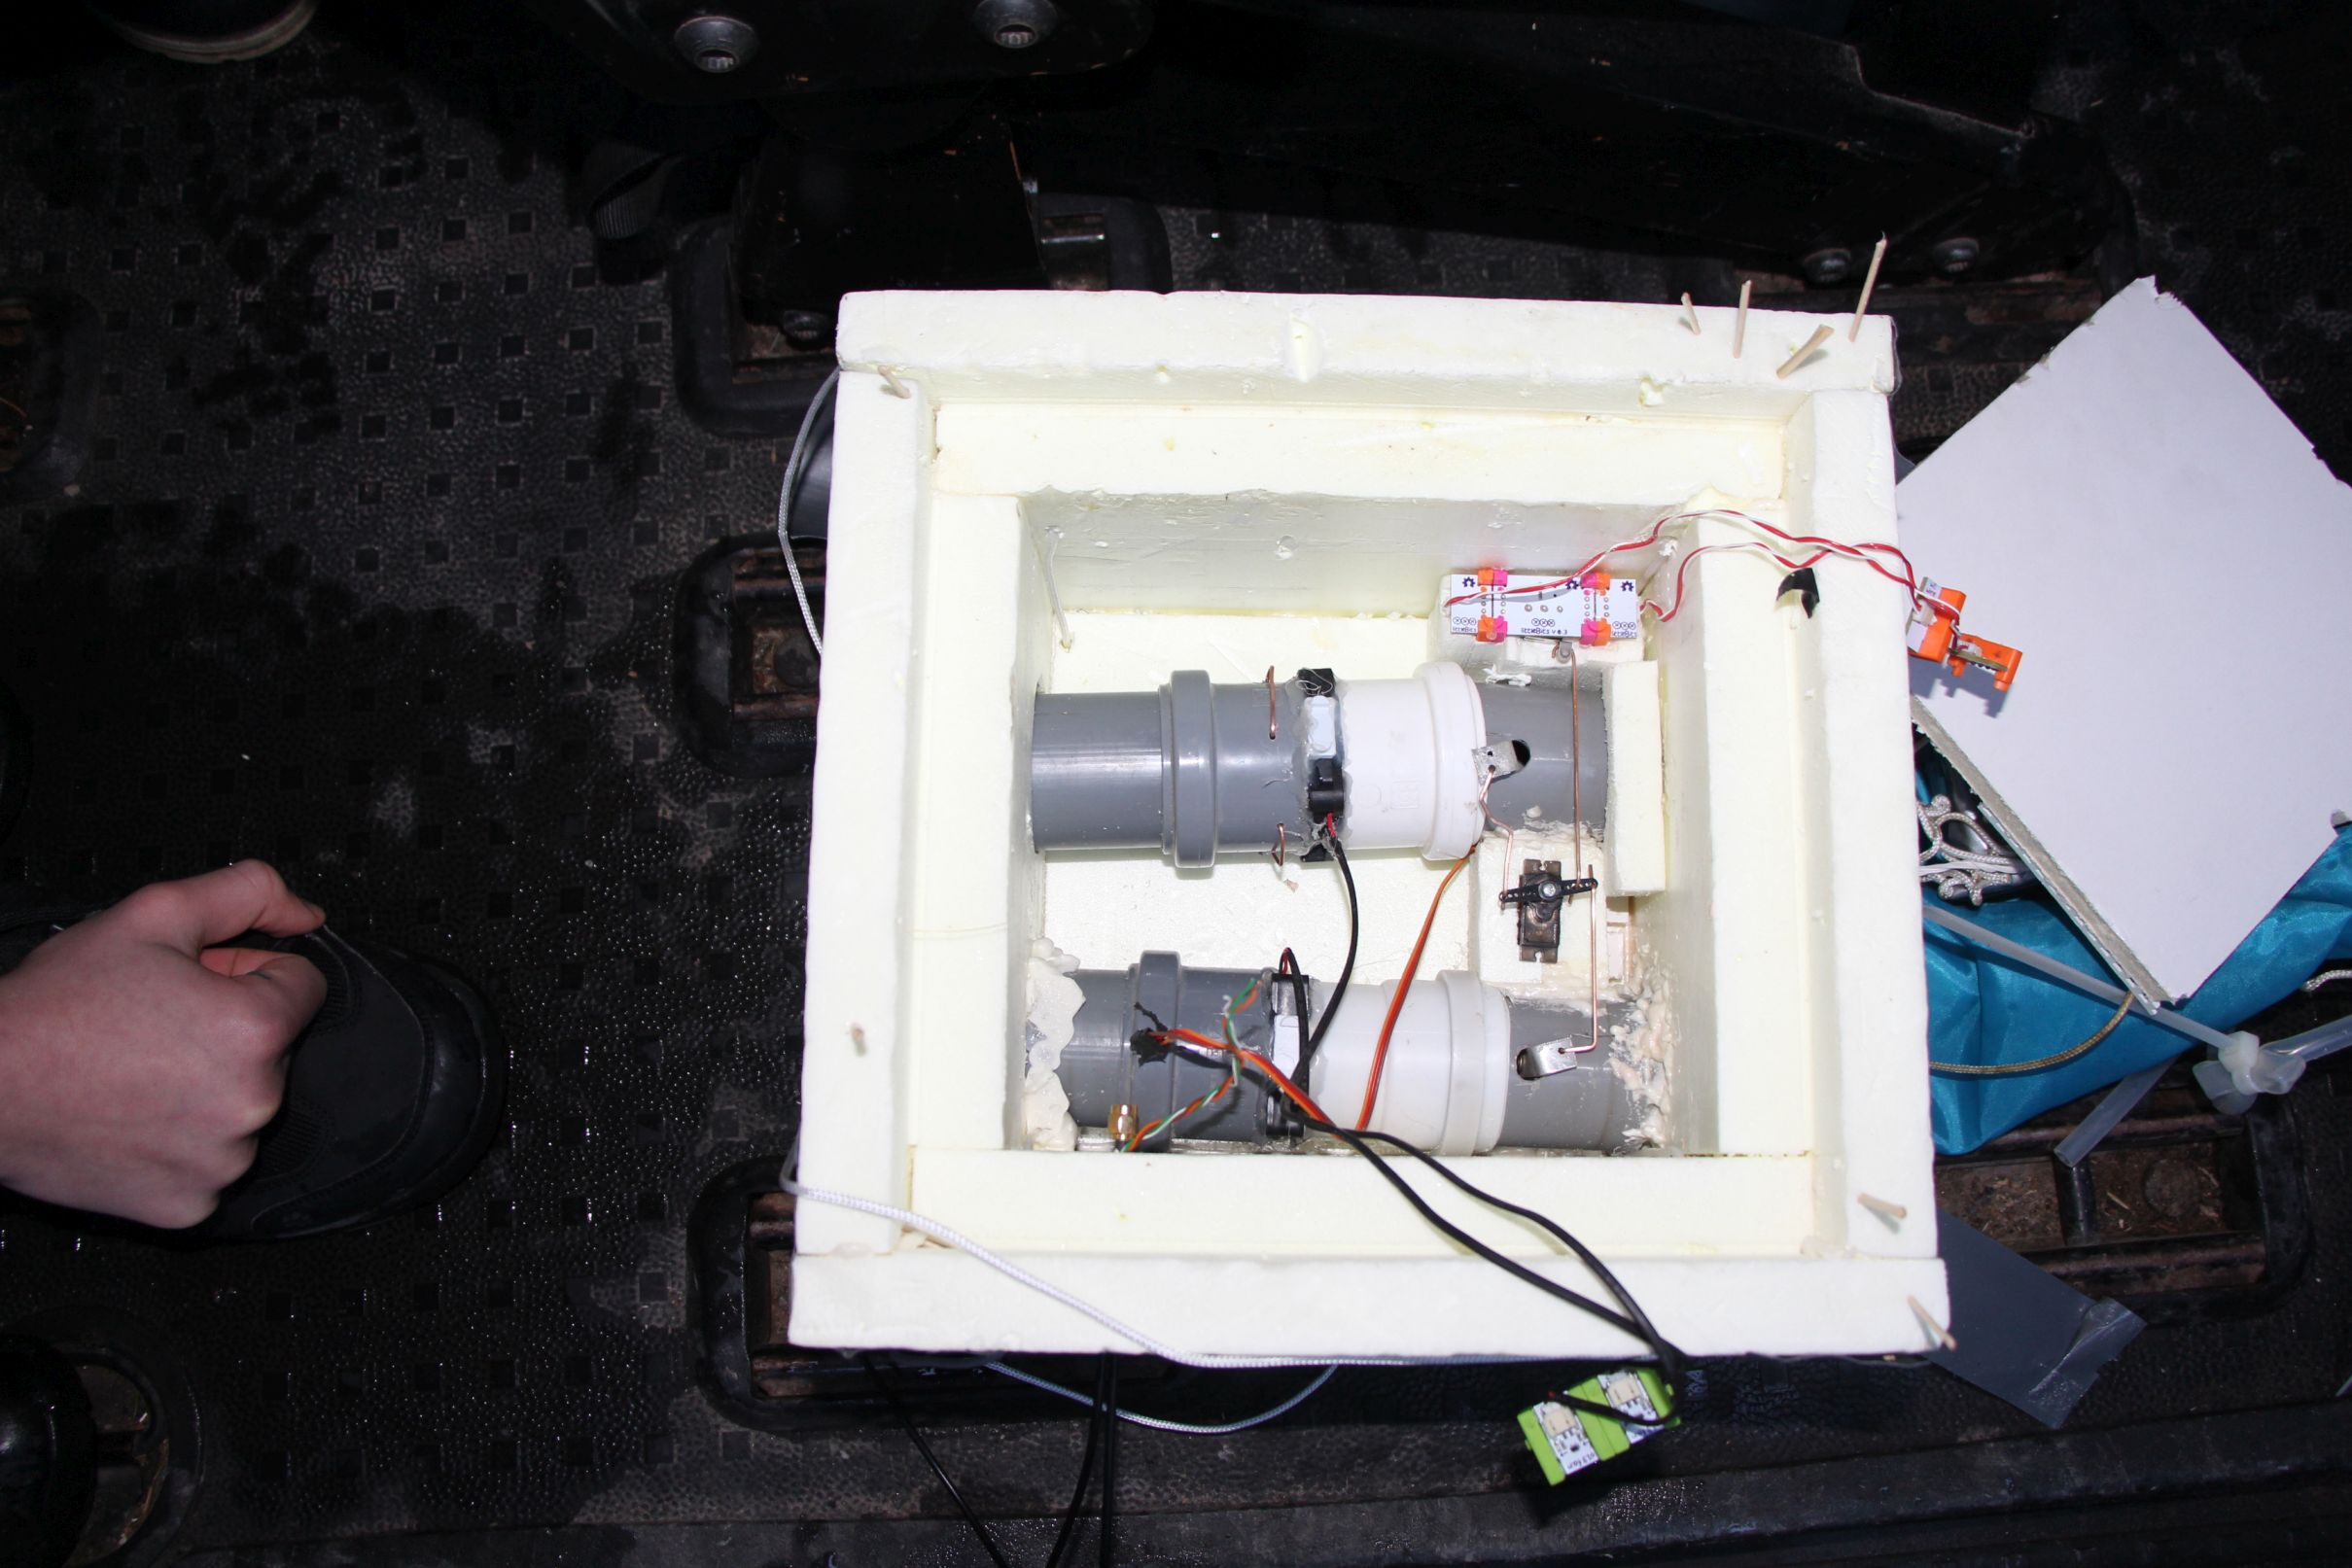
\includegraphics[width=1\textwidth]{PicGra/sond2korrus.jpg}
	\caption{Pilt sondist}
	\allikas{\url{http://pildid.real.edu.ee/main.php?g2_itemId=84935}}
	\label{sond1}
\end{figure}
Sondi mass oli \SI{1375}{g}. Sondi välimus on joonisel \ref{sond2}. Sondist tuli välja nii raadio- kui ka GPS-antenn ning ka andur BME280. Sondi peale oli kinnitatud langevari. Eraldi korpuses asus GPS jälgija GL300, mida kasutati pärast sondi leidmisel. Lennuks kasutati Hwoyee \SI{600}{g} õhupalli.
\begin{figure}[h]
	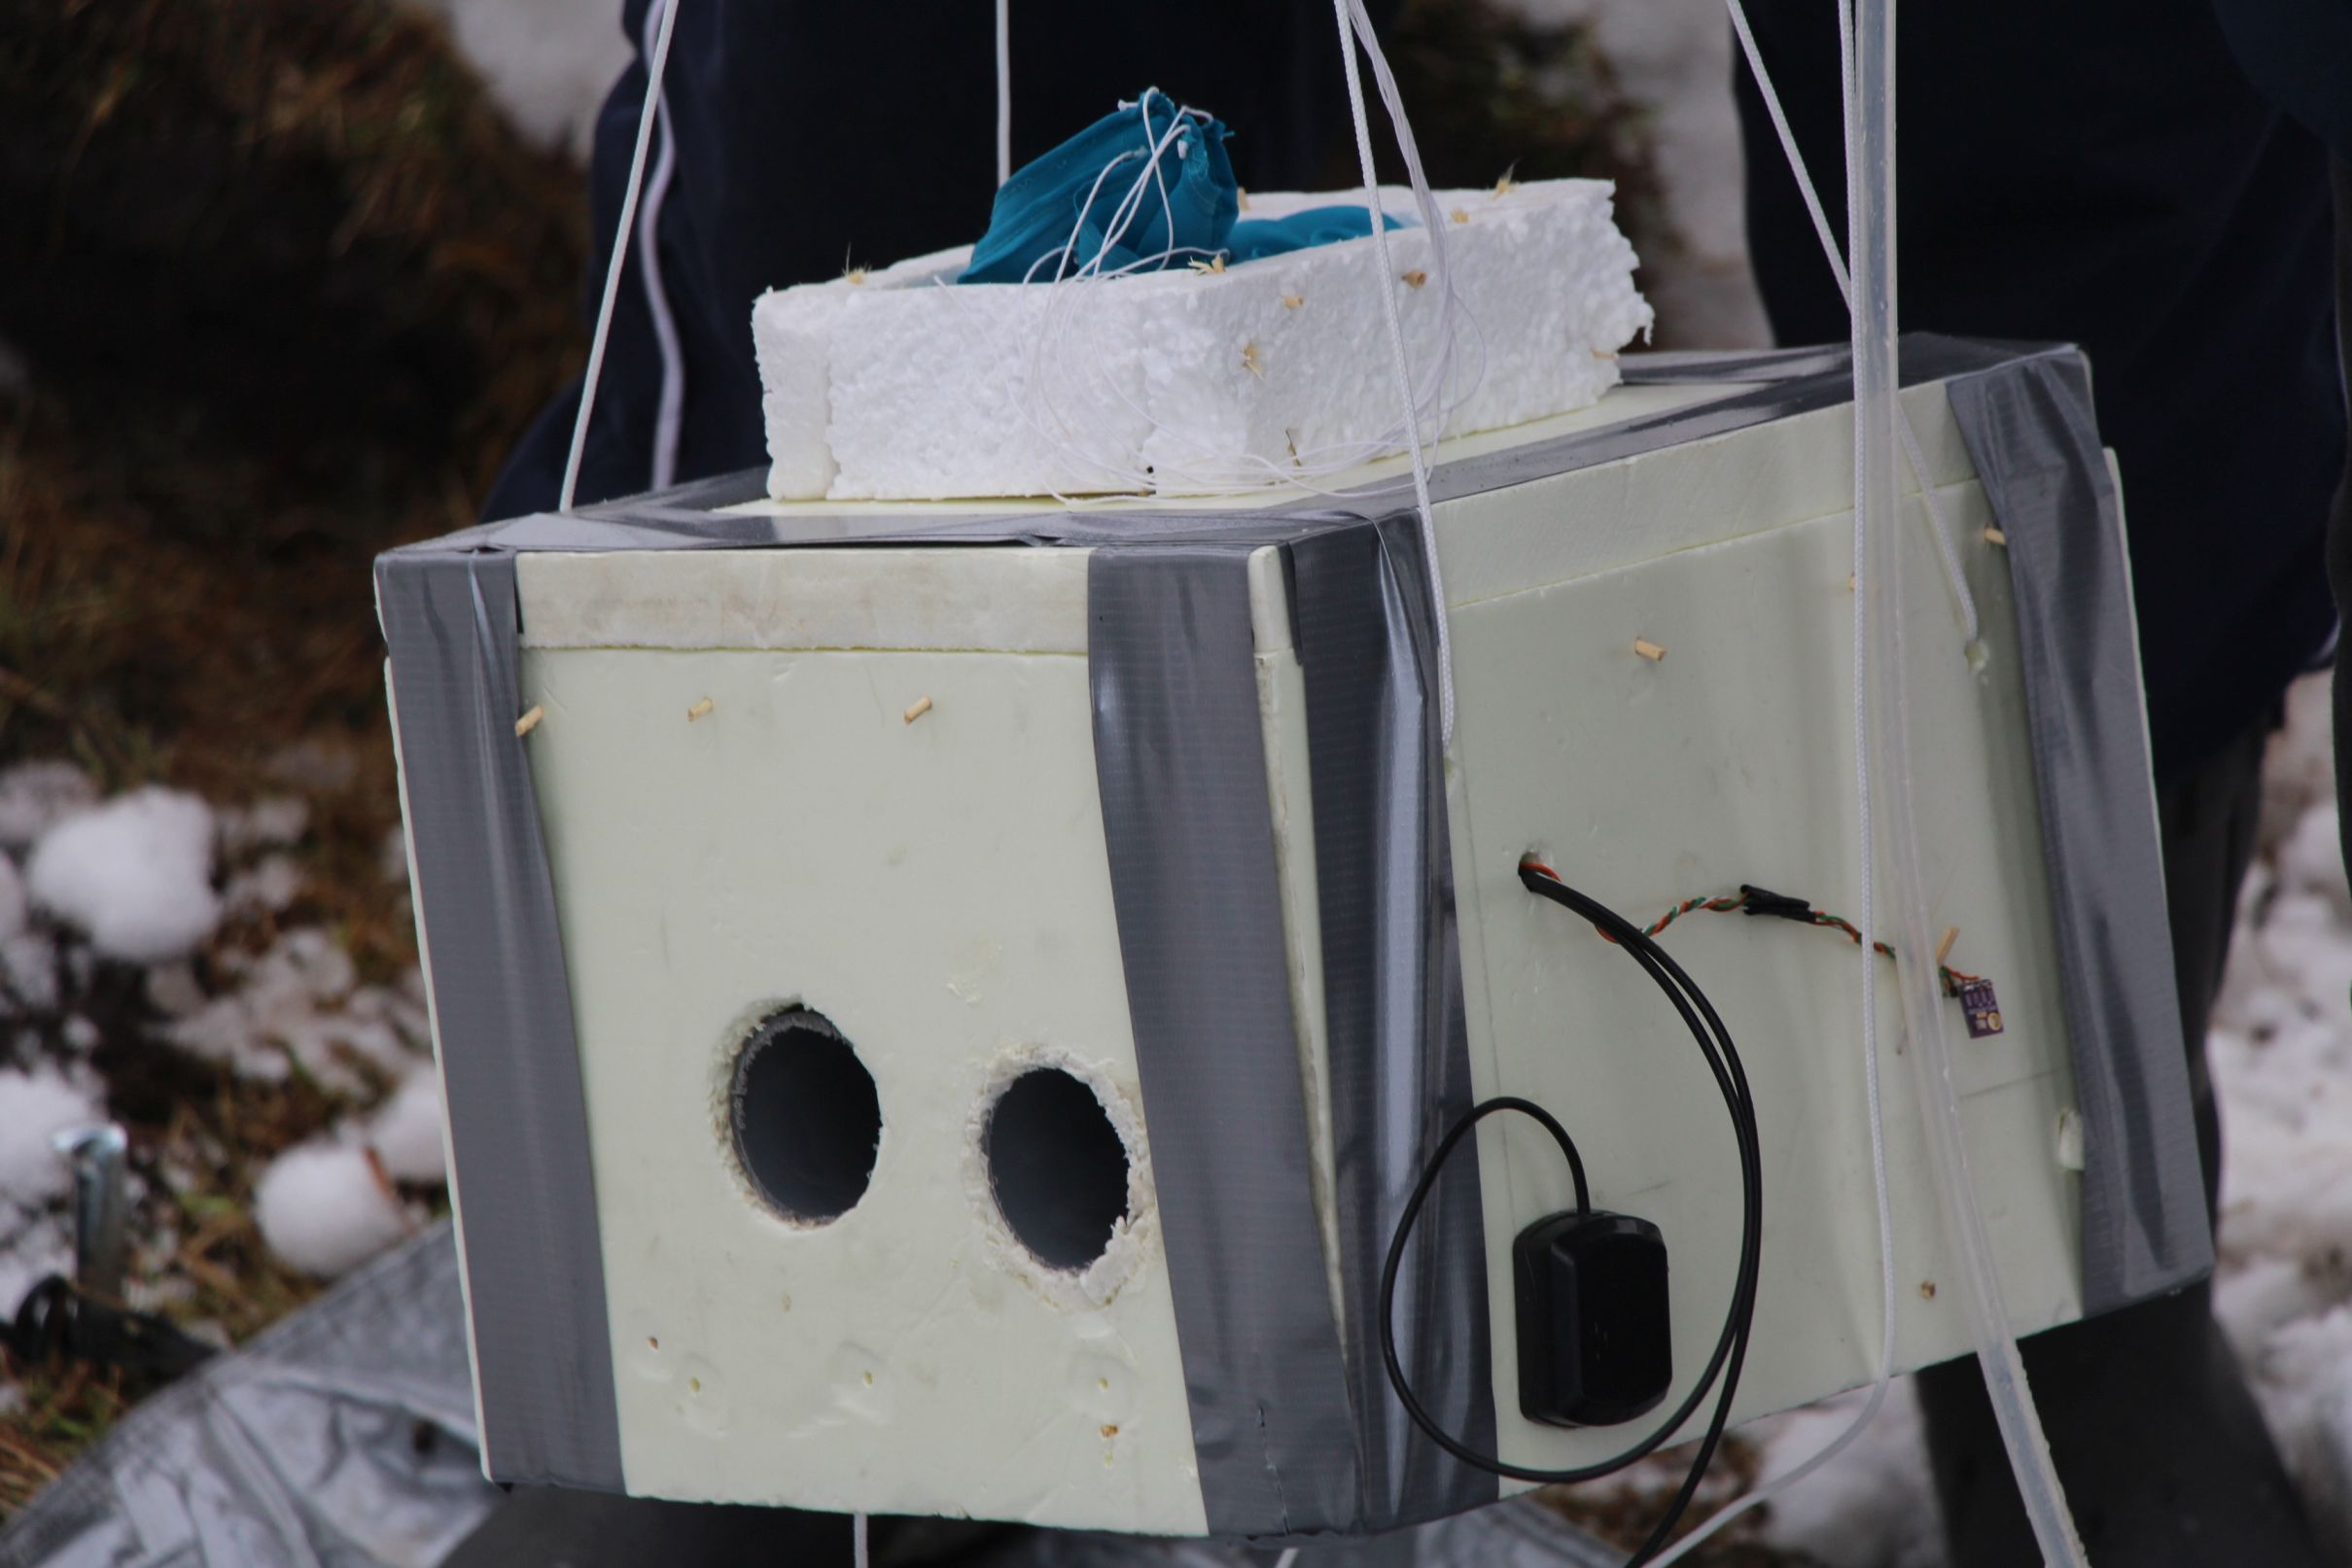
\includegraphics[width=1\textwidth]{PicGra/sond.jpg}
	\caption{Pilt sondist}
	\allikas{\url{http://pildid.real.edu.ee/main.php?g2_itemId=84935}}
	\label{sond2}
\end{figure}

Autor vastutas kogu tehnika töötamise eest. Autor paigaldas sondi esimesele korrusele kogu vajaliku tehnika, ühendas sensori ja mootori Raspberry Pi külge ja seadis sondi lennuvalmis. Autor kirjutas arvutiprogrammi, mis mõõtis andmeid, saatis andmeid ja avas õigel hetkel klapid tolmu kogumiseks. Autor seadis üles arvuti ja antenni, millega saadi lennu käigus jooksvalt andmeid kätte.

\section{Katseseadmed}
Kogu tehnilist poolt juhtis Raspberry Pi arvuti. Raspberry külge kinnitati lisaks Pi In The Sky (PITS) plaat. PITS plaadi külge kinnitati GPS-antenn, mille järgi saadi teada geograafilisi koordinaate, kõrgust ja kellaaega, ja raadioantenn, millega saadeti mõõdetud andmed maapinnale, et jooksvalt jälgida sondi lendu. Raspberry Pi arvuti küljes oli temperatuuri andur, millega mõõdeti sisetemperatuuri. Raspberry Pi külge kinnitati BME280 sensor. Sensor mõõtis temperatuuri, õhurõhku ja õhuniiskust. Sensor viidi juhtmetega sondist välja, et mõõta välistingimusi, mitte sondi sisetingimusi. Raspberry Pi külge kinnitati ka väike mootor. Mootori pööramisel avanesid klapid ja sulgus vooluring, millega pandi ventilaatorid tööle. Sondi sees oli akupank, mis oli ühe juhtmega ühendatud Raspberry Pi külge toiteks ja teise juhtmega ühendatud vooluringi, kus asusuid ventilaatorid.

Andmeid kogus käesoleva uurimistöö autori poolt kirjutatud programm. Programm leidis GPS-antenni kaudu enda asukoha ja lisas sinna sensori poolt mõõdetud tulemused. Saadud andmerea salvestas programm logifaili ja lisaks saatis PITS plaadi külge kinnitatud raadioantenni kaudu info laiali. Programm kontrollis igal ajahetkel kõrgust ja kui see ületas \SI{20}{km}, siis saatis programm signaali mootorile, pöörates mootorit, millega hakkati tolmu koguma. Kui kõrgus oli sellest väiksem, siis pandi mootor tagasi algasendisse.

Raadiosignaal saadi kätte raadioantenniga, mille signaal edastati arvutisse. Kasutades tarkvaralist raadiot, muudeti saadud signaal heliks ja suunati virtuaalse helijuhtme abil helikaardi dekodeerimistarkvarra. Seal muuudeti heli tekstiks, kust oli võimalik välja lugeda mõõdetud andmed.

Eraldi väikessesse korpusesse pandi GL300 jälgija ja kinnitati suurema korpuse külge. Jälgija pandi eraldi korpusesse, et signaalid erinevate seadmete vahel ei hakkaks segama üksteist. Jälgija kasutas GPS'i, et leida oma asukohta ja siis saatis selle mobiilset andmesidet kasutades Internetti, kust oli võimalik teada saada jälgija asukohta. Seade pandi sondiga kaasa, et pärast maandumist lihtsalt sond üles leida. Kuna nõrk raadiosignaal ei levi hästi läbi metsa, siis raadiosignaali abil leida sondi üles maandumiskohast on aeganõudev. Kuid kuna teatud kõrgusel kaob ära mobiilne võrk, siis oli võimalik sellist meetodit kasutades jälgida sondi lennu alguses ja lennu lõpus, kui sond oli maapinna lähedal.

\section{Katse läbiviimine}
Lennu start oli planeeritud kell 11:00 10. veebruaril 2019. Libedad teeolud külavaheteedel pikendasid stardikohale jõudmise aega, lükates starti edasi. Varblasse jõudes otsiti sobiv koht, kus oli stardi jaoks vajalik vaba ala ja lage ala ida suunas, et sondi oleks võimalik lennates kaua jälgida, kuna tugev tuul puhus läänest. Õhupalli täideti balloonis olnud heeliumiga. Balloonis oli \SI{4000}{l} heeliumi. Soovitud heeliumikogus mõõdeti ballooni küljes oleva rõhumõõdikuga. Lennus kasutati \SI{600}{g} massiga lateksist õhupalli. Õhupalli täitmiseks võeti plastmassist pastaka toru korpus ja selle ümber mässiti tihedalt õhupalli suu. Kinnituseks kasutati nipukaid. Pastaka teise otsa ühendati voolik, mis oli ühendatud ballooniga. Pastakat kasutati, et oleks võimalik teha võimalikult tihe ühendus vooliku ja õhupalli vahel ilma, et sulguks heeliumi liikumine balloonist õhupalli. Peale õhupalli täitmist volditi voolik õhupalli lähedalt mitmekordselt kokku ja kinnitati see nipukatega. Seejärel lõigati voolik läbi. Pika nööriga kinnitati sond õhupalli suu külge. Kokku pandi õhupalli umbes \SI{2800}{l} heeliumi. Tugeva tuule tõttu pidi õhupalli väga maa lähedal täitma ja lisaks kätega õhupalli kinni hoidma. Lisaks enne lõplikku vooliku läbilõikamist kontrolliti, kas õhupall suudab sondi õhku tõsta ja hinnati tõstejõu piisavust.

Vahetult enne lendu helistati Lennuametisse ja küsiti viimast kinnitust lennuks. Lennu start toimus kell 11:51. Sond kadus pilvise ilma tõttu mõne minutiga vaateväljast. Raadiosidet suudeti hoida umbes \SI{20}{min}. Peale seda polnud võimalik puhast signaali kätte saada. Siis kadus GPS jälgija ühendus mobiilisideme teenuspakkujaga kõrguse tõttu. Peale sideühenduse kadumist hakati liikuma ennustatava maandumiskoha poole Paidesse. Peale maandumist ühendas GPS jälgija ennast uuesti teenusepakkuja võrku ja saadi teada sondi kukkumise asukoht. Sond maandus kell 14:06 Paide lähedal paarkümmend meetrit Tallinn-Tartu maanteest. Sondi maandumisest saadi teada umbes \SI{15}{min} peale seda, kui kontrolliti sondi asukohta GPS jälgija kaudu.






\chapter{Katseandmete analüüs}
Andmete analüüsimisks kasutati autori poolt kirjutatud programmi. Programm aitas suurest andmekogust välja sorteerida vajalikud andmed ja kontrollida katseandmete kokkulangemist teoreetiliste seostega.

\section{Lennu asukohaline ülevaade}

\begin{figure}[h]
	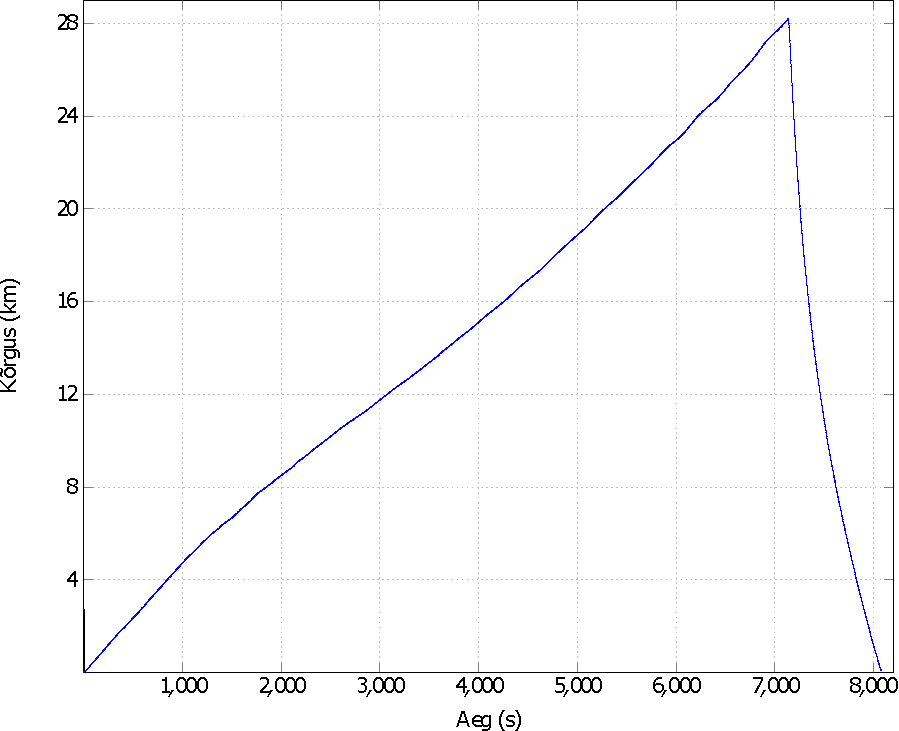
\includegraphics[width=1\textwidth]{PicGra/kõraeg.pdf}
	\caption{kõrguse sõltuvus ajast}
	%\allikas{Minu programm}
	\label{kõraeg}
\end{figure}

Joonisel \ref{kõraeg} on näha sondi kõrguse muutumist ajas. Kokku kestis lend \SI{8083}{sekundit}, ehk 2 tundi, 14 min ja 43 sekundit. Selle aja jooksul tehti kokku 2460 mõõtmist. Mõõtmised on tehtud sekundilise täpsusega iga 3 või 4 sekundi tagant. Keskmiselt tehti mõõtmisi iga \SI{3.29}{s} tagant.

Tõusmisel oli sondil ühtlane tõusukiirus. Keskmine kiirus tõustes oli \SI{3.95}{m/s}. Laskudes kiirus varieerus. Peale kukkumise algust langes sond kiiresti väikese õhutiheduse tõttu. Keskmine kiirus peale langemise algust esimesel \SI{4}{km} oli \SI{78}{m/s}. Keskmine kiirus vahetult enne kokkupõrget maaga oli \SI{14}{m/s}. Kogu kukkumise keskmine kiirus oli \SI{29.8}{m/s}.

Joonisel \ref{trajektoor} on näha sondi liikumise trajektori. Värvidega on näidatud sondi kõrgus. Roosa on kõrgusel \SI{0}{km} kuni \SI{4}{km}, lilla on kõrgusel \SI{4}{km} kuni \SI{8}{km}, sinine on kõrgusel \SI{8}{km} kuni \SI{12}{km}, roheline on kõrgusel \SI{12}{km} kuni \SI{16}{km}, kollane on kõrgusel \SI{16}{km} kuni \SI{20}{km}, oranž on kõrgusel \SI{20}{km} kuni \SI{24}{km} ja punane on kõrgusel \SI{24}{km} kuni suurima kõrguseni, milleks oli \SI{28.188}{km}. Tõusmisel läbis sond suure horisontaalse nihke, milleks oli \SI{109.86}{km}. See tähendab, et andmed pole tõustes kogutud ühe vertikaalse joone peal, vaid üpris laia ala peal. Allakukkumisel läbis sond horisontaalselt ainult \SI{14.5}{km} ja seda palju väiksema ajaga. Seega kukkumisel mõõdetud andmed on tehtud väikese ajaga umbes sama vertikaalse joone peal.
\begin{figure}[h]
	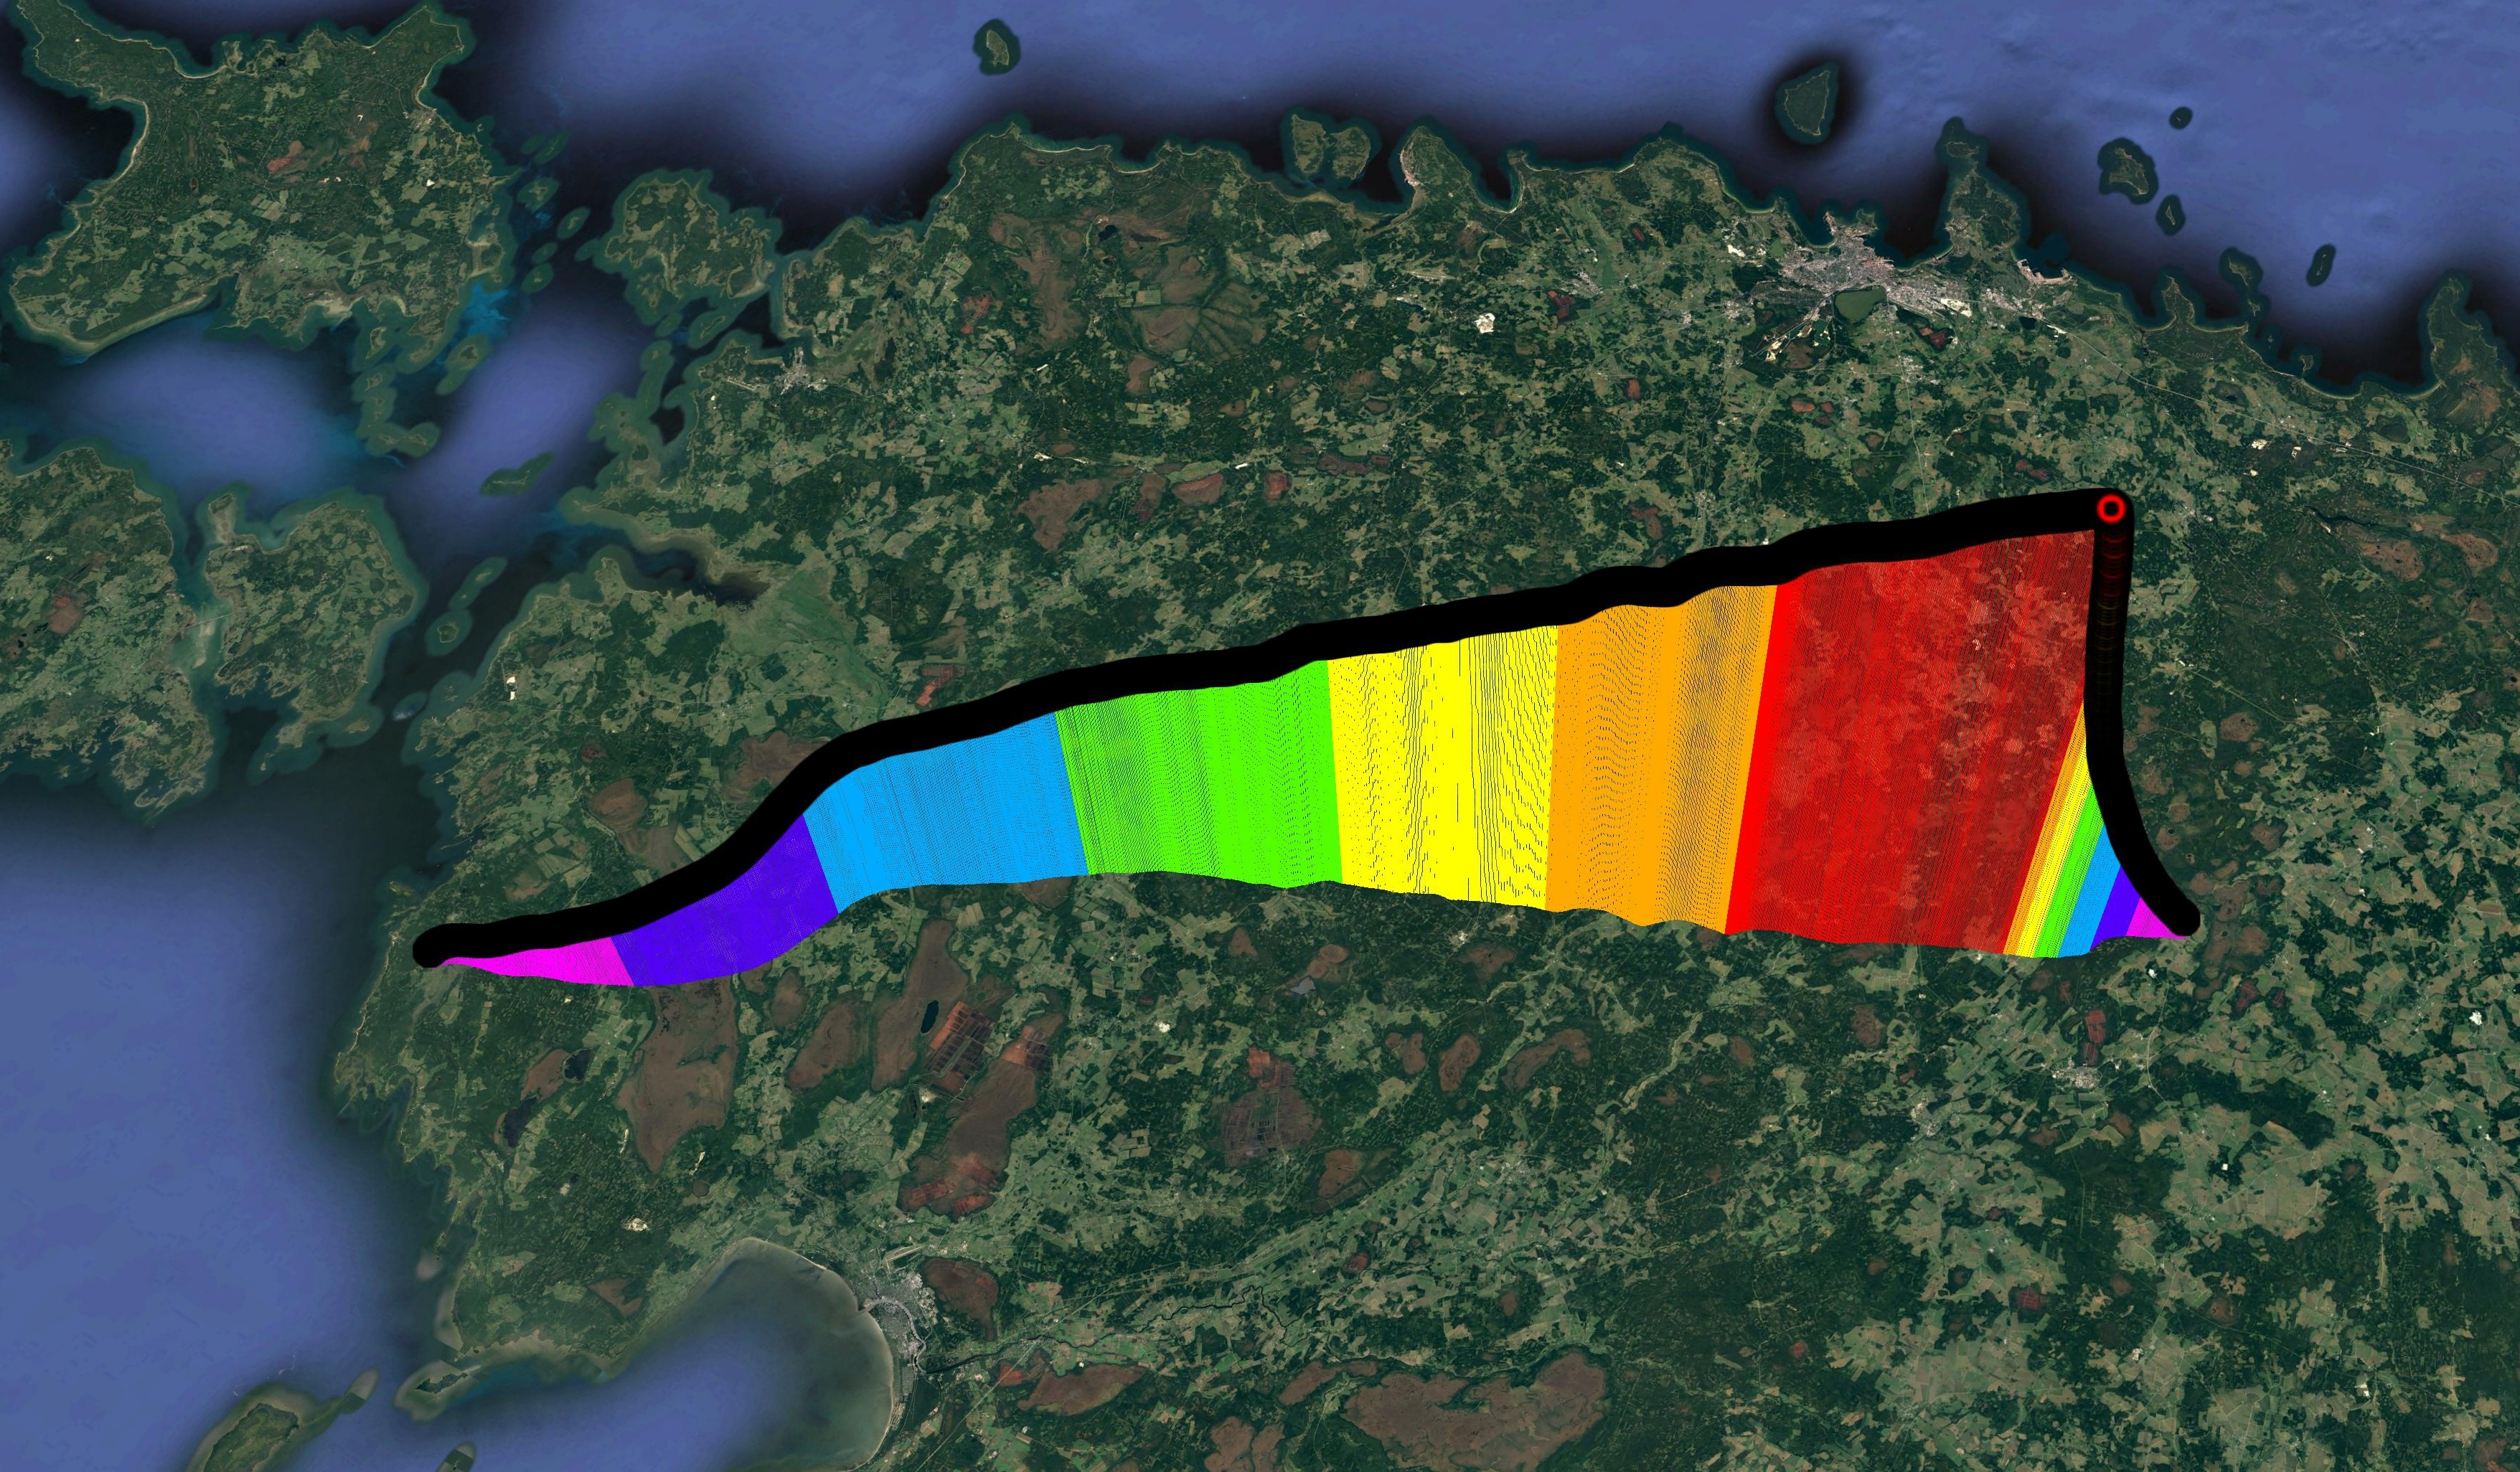
\includegraphics[width=1\textwidth]{PicGra/teekond.jpg}
	\caption{Sondi trajektoor}
	\allikas{Autori erakogu ja Google Earth}
	\label{trajektoor}% Selle järgi viidatakse, see rida peab olema pärast \caption
\end{figure}

\section{Temperatuuri muutus kõrgusega}
Joonisel \ref{TempKõrgus} on näha temperatuuri näit kõrguse muutumisel. Joonisel on kaks joont, sest andmeid mõõdeti igalt kõrguselt kaks korda, sondi tõusmisel ja sondi laskumisel. Lennu stardi ajal oli kõrgem temperatuur, kui lennu lõppemise ajal.

\begin{figure}[h]
	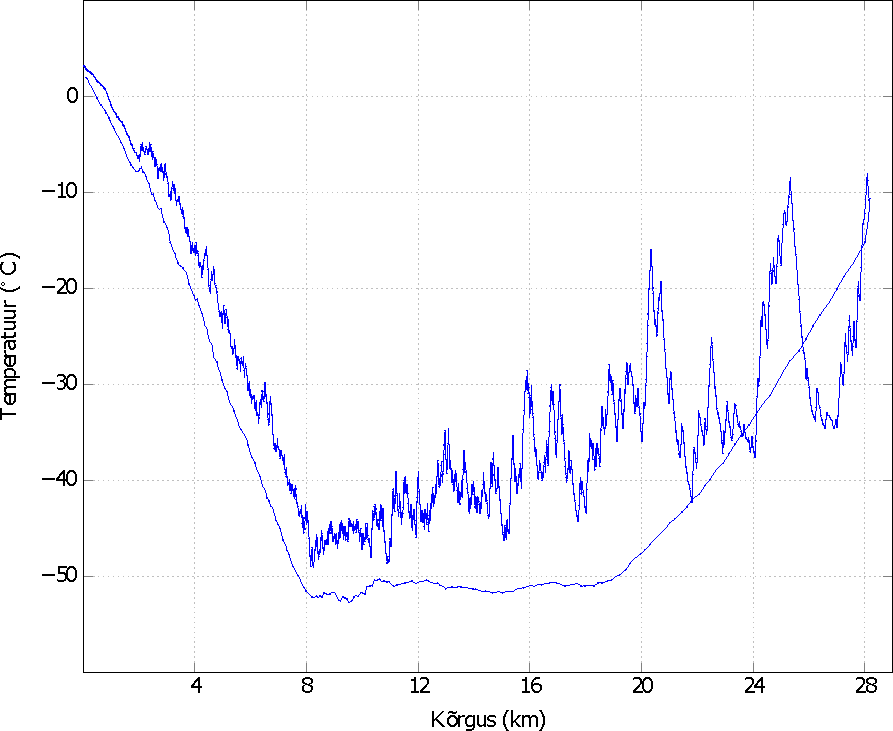
\includegraphics[width=1\textwidth]{PicGra/tempkõr.pdf}
	\caption{Temperatuuri sõltuvus kõrgusest}
	%\allikas{Minu programm}
	\label{TempKõrgus}% Selle järgi viidatakse, see rida peab olema pärast \caption
\end{figure}

Joonisel on näha, kuidas temperatuur kõigub, mitte ei muutu ühtlaselt. See on tingitud päikesekiirgusest. Kui sensor on Päikese
poole, siis soojendab Päike sensorit. Kui sensor on sondi varjus, siis peale mahajahtumist mõõdab sensor jälle tegelikku õhutemperatuuri. Sensor ei mõõda kunagi madalamat temperatuuri, kui tegelik õhu temperatuur. Kõrguse kasvades muutub temperatuuri kõikumise amplituud suuremaks. See on tingitud madalast rõhust. Kui õhk hõreneb, siis hakkab sondi temperatuuri rohkem mõjutama Päike, kui õhk ise.

Kukkumise alguses on sensor pikalt olnud Päikese poole ja soojenenud. Seega sensor kukkumise ajal jahtub, kuid kuna nende kõrguste juures kõrguse vähenemisel langeb ka temperatuur, ei saavuta sensor välisemperatuuri varem kui \SI{20}{km} kõrgusel maast. Sel ajal on näha sujuvat temperatuuri muutust. Sensori mitte ülessoojenemist kukkumisel võib põhjendada mitut moodi. Sond võis kukkumisel hakata tugevalt pöörlema, mille tõttu polnud sensoril aega üles soojeneda. Kogu lennu vältel liikus sond külgtuultega samal kiirusel ja sama suunaga. Seega sondile mõjusid tuuled, mis tulenevad üles liikumisest ja allakukkumisest. Kuna kuni \SI{20}{km}'ni kukkus sond keskmise kiirusega \SI{70}{m/s}, siis jahutas tuul sensorit.

Kõrgemal kui \SI{8}{km} hakkab temperatuur kõrguse kasvades suurenema. See on tingitud osoonikihis neelduvast UV kiirgusest. Kuna järgnevalt uuritakse, kas temperatuur muutub adiabaatilise protsessi käigus, siis vaadeldakse ainult umbes esimest \SI{8}{km}. Täpseks kõrguseks valiti \SI{8154}{m}. Sellel kõrgusel tehti viimane mõõtmine, mis oli temperatuurigraafiku viimane lokaalne miinimum, peale mida hakkas temperatuur jälle tõusma. Kuna graafik on ebatasane, vastab lokaalne miinimum kõige paremini tegelikule temperatuurile. Sama kõrgus valiti ka kukkumisel.

Joonisel \ref{tempkõrtrop} on anomaalia. Umbes \SI{2}{km} kõrgusel on nii laskumisel kui ka tõusmisel näha kõrguse suurenemisel väikest temperatuuri muutust. Kuna see toimub nii tõusmisel kui ka kukkumisel, siis on see suure tõenäosusega tegelik temperatuuri muutus ja mitte sensori viga või muud sellist.
\begin{figure}[h]
	\includegraphics[width=1\textwidth]{PicGra/tempkõrtrop.pdf}
	\caption{Temperatuuri sõltuvus merepinnast kuni kõrguseni \SI{8}{km}}
	\allikas{Autori erakogu}
	\label{tempkõrtrop}% Selle järgi viidatakse, see rida peab olema pärast \caption
\end{figure}

Vaadates joonist \ref{humkõrtrop} on näha, et kuni \SI{2}{km} kõrguseni on õhuniiskus ühtlaselt kõrge. Kuid peale \SI{2}{km} on näha, et õhuniiskus langeb tugevalt. Õhuniiskus langes, kuna sond väljus pilvedest ning temperatuur tõusis. Pilvedest väljumist saab ka tõestada temperatuuri kõikumise algusega. Esimesed \SI{2}{km} temperatuur ei kõikunud, kuna Päikest ei paistnud sondile peale. Pilvedest väljudes hakkas aga Päike mõjutama sensori lugemit. Kuna osa mõõtmisi tehti pilvede sees ja osa pilvedest väljas, otsustati vaadelda temperatuuri muutumist eraldi pilvedest madalamal ja pilvedest kõrgemal.
\begin{figure}[h]
	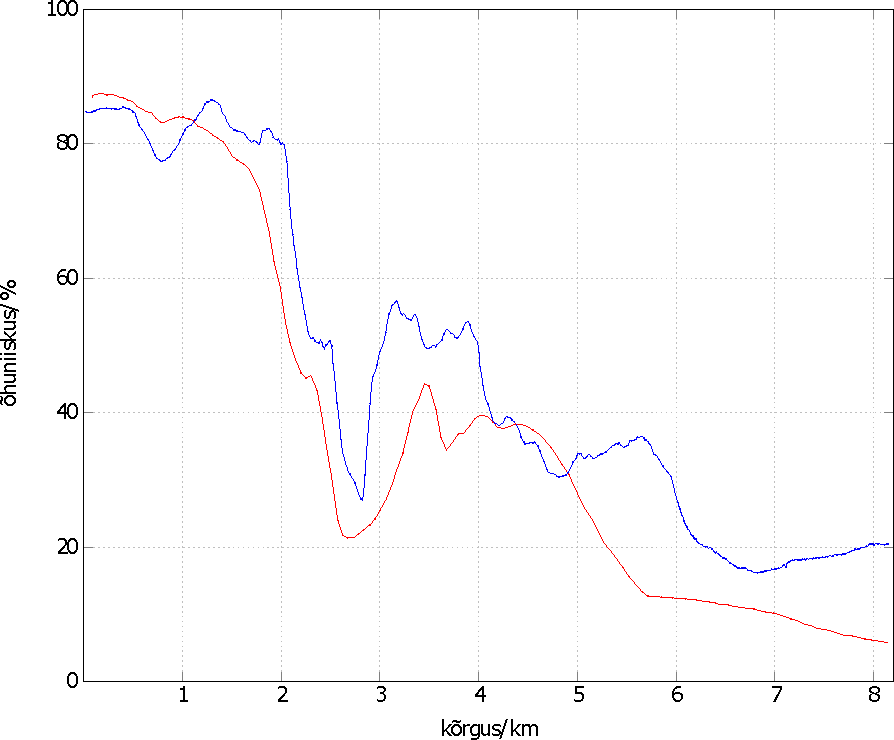
\includegraphics[width=1\textwidth]{PicGra/humkõrtrop.pdf}
	\caption{Õhuniiskuse sõltuvus kõrgusest merepinnast kuni kõrguseni \SI{8}{km}}
	\allikas{Autori erakogu}
	\label{humkõrtrop}% Selle järgi viidatakse, see rida peab olema pärast \caption
\end{figure}

Järgnevalt leitakse temperatuuri muutusele kõrgusega parim lineaarne seos:
\begin{equation*}
T(z) = T_0 + \Gamma z.
\end{equation*}
kus $T_0$ on temperatuur algpunktis ja $\Gamma$ on temperatuurigradient, ehk temperatuuri muutus kõrguse kasvades. Lineaarse seose leidmiseks kasutati vähimruutude meetodit, mis avaldub järgnevalt:
\begin{equation*}
\Gamma = \frac{\sum_{i=1}^{n}(z_i - \overline{z})(T_i - \overline{T})}{\sum_{i=1}^{n}(z_i - \overline{z})^2}
\end{equation*}
\begin{equation*}
T_0 = \overline{T} - \Gamma \overline{z}
\end{equation*}
kus $z$ on kõrgus ja $T$ on temperatuur \parencite[252-285]{mat}.

Pilvede sees vaadati temperatuure õhupalli tõustes kuni \SI{2010}{m} meetrini. Sellel kõrgusel tehti viimane mõõtmine, peale mida temperatuur tõusis pilvedest väljumise tagajärgel. Samal põhjusel valiti laskumisel viimaseks andmepunktiks \SI{1926}{m} kõrgusel mõõdetud andmepunkt.

Joonisel \ref{tempkõrtroppilvlin} on näha temperatuuri muutust selles vahemikus. Laskumisel on temperatuurigradient $\Gamma =  \SI{-5.53009}{\degreeCelsius/km}$ ning temperatuur algpunktis on $T_0 = \SI{2.12611}{\degreeCelsius}$. Tõusmisel merepinnast kuni kõrguseni \SI{2}{km} on näha kahte erinevat lineaarset temperatuuri muutust. Merepinnast kuni kõrguseni \SI{793}{m} on temperatuurigradient $\Gamma =\SI{-3.19233}{\degreeCelsius/km}$ ja temperatuur algpunktis $T_0 = \SI{3.16728}{\degreeCelsius}$. Kõrguste vahemikus \SI{808}{m} kuni \SI{2010}{m} on temperatuuri gradient $\Gamma =\SI{-5.73645}{\degreeCelsius/km}$ ja temperatuur algpunktis $T_0 = \SI{0.360244}{\degreeCelsius}$.

\begin{figure}[h]
	\includegraphics[width=1\textwidth]{PicGra/tempkõrtroppilvlin.pdf}
	\caption{Temperatuuri sõltuvus kõrgusest merepinnast kuni kõrguseni \SI{2}{km}}
	\allikas{Autori erakogu}
	\label{tempkõrtroppilvlin}% Selle järgi viidatakse, see rida peab olema pärast \caption
\end{figure}


Tõusmisel valiti algpunktiks \SI{2565}{m} kõrgusel mõõdetud andmepunkt. See on esimene andmepunkt, alates \SI{2010}{m} kõrgusel asuvast andmepunktist, kus on madalam temperatuur, kui \SI{2010}{m} kõrgusel mõõdetud temperatuur. Laskumisel valiti algpunktiks \SI{2136}{m} kõrgusel mõõdetud andmepunkt. See on esimene andmepunkt, alates \SI{1926}{m} kõrgusel mõõdetud andmepunktist, kus on madalam temperatuur kui \SI{1926}{m} kõrgusel mõõdetud temperatuur. Antud vahemikus olevad mõõtmised on kuvatud joonisel \ref{tempkõrtroplin}.

Tõusmisel on temperatuurigradient $\Gamma =\SI{-7.13399}{\degreeCelsius/km}$ ja temperatuur algpunktis $T_0 = \SI{-5.4533}{\celsius}$. Laskumisel oli temperatuurigradient $\Gamma =\SI{-7.67992}{\degreeCelsius/km}$ ja temperatuur algpunktis $T_0 = \SI{-7.26635}{\celsius}$.

\begin{figure}[h]
	\includegraphics[width=1\textwidth]{PicGra/tempkõrtroplin.pdf}
	\caption{Temperatuuri sõltuvus kõrgusest üle \SI{2}{km}}
	\allikas{Autori erakogu}
	\label{tempkõrtroplin}% Selle järgi viidatakse, see rida peab olema pärast \caption
\end{figure}

Tõusmise graafik on kõikuv, mille on põhjustanud päikesekiirgus. Kuna Päike soojendas, siis sensor mõõtis tegelikust kõrgemat temperatuuri. Kui sensor jahtus, siis mõõtis sensor tegelikku temperatuuri. Kasutades asjaolu, et sensor ei mõõtnud tegelikust madalamat temperatuuri, võib eemaldada kõik kõrvalekalded. Andmeid hakati madalamast kõrgusest vaatama nii, et temperatuur pidevalt langeks. Kui kõrguse suurenedes temperatuur tõuseb, eemaldati järjest kõik andmepunktid, kuni jõuti andmepunktini, mis oli madalam viimasest võrdluspunktist. Tulemus on joonisel \ref{tempkõrtroplinstalin}. Temperatuurigradient on $\Gamma =\SI{-7.23193}{\degreeCelsius/km}$ ja temperatuur algpunktis $T_0 = \SI{-5.961}{\celsius}$.

\begin{figure}[h]
	\includegraphics[width=1\textwidth]{PicGra/tempkõrtroplinstalin.pdf}
 	\caption{Temperatuuri sõltuvus kõrgusest üle \SI{2}{km}}
 	\allikas{Autori erakogu}
 	\label{tempkõrtroplinstalin}% Selle järgi viidatakse, see rida peab olema pärast \caption
\end{figure}

Tabelis \ref{tabel1} on kokkuvõttev tabel selles osas mõõdetud andmetest. Kui kasutada valemit \ref{eq12}, saab temperatuurigradienti kasutades leida veeauru massiosakaalu õhus, saades valemiks
\begin{equation*}
\omega = \frac{g + c_o}{\Gamma(c_o-c_v)}.
\end{equation*}
\begin{table}[htb]
	\caption{Temperatuurigradiendid erinevatel kõrgustel}
	\label{tabel1}
	\begin{tabular}{r|r|r|r|r}
		\hline
		alguspunkti kõrgus & lõpppunkti kõrgus & tõus/langus & $T_0$ & $\Gamma$ \\
		\hline
		22 & 793 & tõus & 3.16728 & -3.19233 \\
		808 & 2010 & tõus & 0.360244 & -5.73645 \\
		2565 & 8154 & tõus & -5.961 & -7.23193 \\
		89 & 1926 & langus & 2.12611 & -5.53009 \\
		2136 & 8154 & langus & -7.26635 & -7.67992
	\end{tabular}
\end{table}

Järgnevalt arvutatakse välja veeauru massiosakaal erinevatel kõrgusvahemikel. Kõrgusel \SI{22}{m} kuni \SI{793}{m} moodustab veeaur \SI{64.9}{\percent} õhu massist. Kõrgusel \SI{808}{m} kuni \SI{2010}{m} moodustab veeaur \SI{22.2}{\percent} õhu massist. Kõrgusel \SI{2565}{m} kuni \SI{8154}{m} moodustab veeaur \SI{11.1}{\percent} õhu massist. Kõrgusel \SI{89}{m} kuni \SI{1926}{m} moodustab veeaur \SI{24.2}{\percent} õhu massist. Kõrgusel \SI{2136}{m} kuni \SI{8154}{m} moodustab veeaur \SI{8.6}{\percent} õhu massist.


\section{Rõhu muutus kõrgusega}
Joonisel \ref{prekõrg} on näha rõhu muutust kogu lennu jooksul. Rõhu mõõtmistulemused on täpsed (kõrvalekalded on suhteliselt väikesed). Jooniselt on seda raske välja lugeda, aga tegelikult eksisteerib kaks joont. Tõusmisel on rõhk madalam kui langemisel.
\begin{figure}[h]
	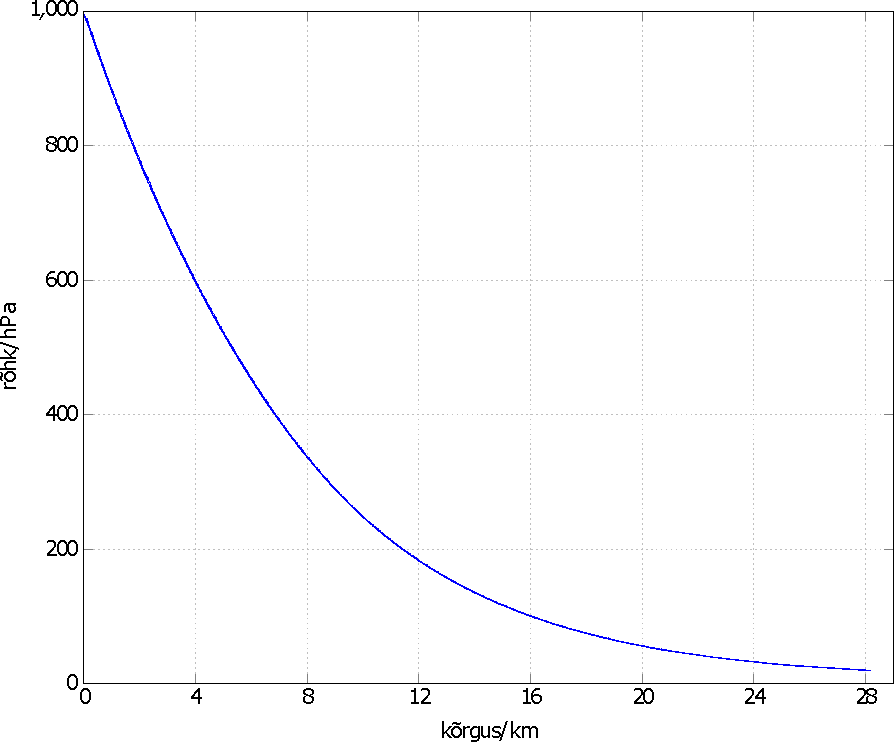
\includegraphics[width=1\textwidth]{PicGra/prekõrg.pdf}
	\caption{Rõhu muutus kõrgusega}
	\allikas{Autori erakogu}
	\label{prekõrg}% Selle järgi viidatakse, see rida peab olema pärast \caption
\end{figure}

Käesolevas osas uuritakse, et kas teooria osas saadud valem, mis kirjeldab rõhu muutust atmosfääris,
\begin{equation}\label{eq14}
p = p_0 \left(1+\frac{\Gamma z}{T_0}\right)^{-\frac{g\mu}{R\Gamma}}
\end{equation}
vastab katseandmetele. Kuna temperatuuri gradient on erinevatel atmosfääri osades erinev, siis vaatame üksikult osi, kus temperatuuri gradient on konstantne. Konstantite väärtused on: $g = \SI{9.80665}{\frac{m}{s^2}}$ , $R = \SI{8.3144598}{\frac{J}{mol*K}}$ ja $\mu = \SI{0.0289647}{\frac{km}{mol}}$. Valemi testimiseks kasutati programmi, mis arvutab algandmete põhjal välja rõhu mõõdetud punkti kõrgusel ja võrdleb sellel kõrgusel mõõdetud rõhuga. Võrdlemise valem on
\begin{equation*}
e = \frac{p_a-p_m}{p_a},
\end{equation*}
kus $p_a$ on arvutatud rõhk ja $p_m$ on mõõdetud rõhk.

Esimene kõrgusvahemik on \SI{22}{m} kuni \SI{793}{m}. Kõrgusel \SI{22}{m} on $p_0=\SI{995.14242}{hPa}$ ja $T_0 = 276.31728$ K. Keskmine erinevus selles kõrgusvahemikus oli \SI{0.515915}{\permil}. Kõrgusel \SI{793}{m} mõõdeti rõhuks \SI{903.92}{hPa} ja arvutati rõhuks \SI{904.276}{hPa}. Järgmise kõrgusvahemiku alguspunktis \SI{808}{m} kõrgusel arvutas programm rõhuks \SI{902.585}{hPa}.

Teine kõrgusvahemik on \SI{808}{m} kuni \SI{2010}{m}. Kõrgusel \SI{808}{m} on $p_0 = 902.01955$ ja $T_0 = 273.510244$ K. Keskmine erinevus selles kõrgusvahemikus oli \SI{0.229426}{\permil}. Kõrgusel \SI{2010}{m} mõõdeti rõhuks \SI{774.026}{hPa} ja arvutati rõhuks \SI{774.777}{hPa}. Järgmise kõrgusvahemiku alguspunktis \SI{2565}{m} kõrgusel arvutas programm rõhuks \SI{721.283}{hPa}. Kui kasutada eelnevas kõrgusvahemikus arvutatud rõhku \SI{808}{m} kõrgusel, mis oli \SI{902.585}{hPa} siis on keskmine erinevus \SI{0.717021}{\permil}. Sellisel juhul on järgmise kõrgusvahemiku alguspunktis \SI{2565}{m} kõrgusel programmi järgi rõhuks \SI{721.735}{hPa}.

Kolmas kõrgusvahemik on \SI{2565}{m} kuni \SI{8154}{m}. Kõrgusel \SI{2565}{m} on $p_0 = 720.86625$ ja $T_0 = 267.189$ K. Keskmine erinevus selles kõrgusvahemikus oli \SI{4.72004}{\permil}. Kõrgusel \SI{8154}{m} mõõdeti rõhuks \SI{329.341}{hPa} ja arvutati rõhuks \SI{332.165}{hPa}. Kui kasutada eelnevas kõrgusvahemikus arvutatud rõhku \SI{2565}{m} kõrgusel, mis oli \SI{721.735}{hPa}, siis on keskmine erinevus \SI{5.91381}{\permil}.

Vaadates langemisel mõõdetud andmeid, on esimene kõrgusvahemik \SI{89}{m} kuni \SI{1926}{m}. Kõrgusel \SI{89}{m} on $p_0=\SI{989.32523}{hPa}$ ja $T_0 = \SI{275.27611}{K}$ ning $\Gamma = \SI{-5.53009}{K/km}$. Keskmine erinevus selles kõrgusvahemikus oli \SI{2.85639}{\permil}. Kõrgusel \SI{1926}{m} mõõdeti rõhuks \SI{786.723}{hPa} ja arvutati rõhuks \SI{784.252}{hPa}. Järgmise kõrgusvahemiku alguspunktis \SI{2136}{m} kõrgusel arvutas programm rõhuks \SI{763.269}{hPa}.

Teisel kõrgusvahemikul \SI{2136}{m} kuni \SI{8154}{m}. Kõrgusel \SI{2136}{m} on $p_0=\SI{765.63645}{hPa}$ ja $T_0 = \SI{265.88365}{K}$ ning $\Gamma = \SI{-7.67992}{K/km}$. Keskmine erinevus selles kõrgusvahemikus oli \SI{4.45647}{\permil}. Kõrgusel \SI{8154}{m} mõõdeti rõhuks \SI{332.17}{hPa} ja arvutati rõhuks \SI{328.404}{hPa}. Kui kasutada eelnevas kõrgusvahemikus arvutatud rõhku \SI{2136}{m} kõrgusel, mis oli \SI{763.269}{hPa}, siis on keskmine erinevus \SI{7.55264}{\permil}.

\section{Mitteadiabaatilised vahemikud}
Atmosfäär ei ole täielikult adiabaatiline. Üks ala, kus atmosfäär ei ole adiabaatiline, on pilvedes, kuna pilvedes toimub veeauru kondenseerumine, mille käigus antakse õhule soojusenergiat. Selline protsess toimub umbes \SI{2}{km} kõrgusel nii tõustes kui ka langedes. Visuaalselt on seda võimalik näha jooniselt \ref{tempkõrtrop}. Nüüd arvutatakse välja, kui palju kondenseerub vett umbes \SI{1}{kg} õhu kohta. Selleks kasutatakse teooria osas leitud valemit
\begin{equation*}
\frac{m_v}{m_a} = \frac{i}{2}\frac{R}{\mu L}\left(T_2- T_0 - \Gamma z\right).
\end{equation*}
Tõustes on temperatuurigradient vahetult enne pilvi $\Gamma = \SI{-5.73645}{K/km}$. Temperatuur kõrgusel \SI{2010}{m} on $T_0 = \SI{-6.76}{\degreeCelsius}$ ja sellest $z = \SI{555}{m}$ kõrgemal kõrgusel \SI{2565}{m} on $T_2 = \SI{-7.33}{\degreeCelsius}$, ning vee aurustumissoojus on $L = \SI{2257000}{\frac{J}{kgs}}$. Kasutades valemis katseandmeid saadakse, et õhust eraldub veeauru
\begin{equation*}
\frac{m_v}{m_a} = 0.83 \frac{g}{kg}.
\end{equation*}
Laskudes on temperatuurigradient vahetult enne pilvi $\Gamma = \SI{-5.53009}{K/km}$. Temperatuur kõrgusel \SI{1926}{m} on $T_0 = \SI{-7.81}{\degreeCelsius}$ ja sellest $z = \SI{210}{m}$ kõrgemal kõrgusel \SI{2136}{m} on $T_2 = \SI{-7.88}{\degreeCelsius}$. Kasutades valemis katseandmeid saadakse, et õhust eraldub veeauru
\begin{equation*}
\frac{m_v}{m_a} = 0.16 \frac{g}{kg}.
\end{equation*}

Ka stratosfääris pole atmosfäär adiabaatiline, sest siseenergat antakse õhule juurde Päikesest tuleva UV kiirguse neeldumisel. Seda on visuaalselt näha jooniselt \ref{TempKõrgus}, kus alates umbes \SI{8}{km}'ist alates temperatuur kasvab. Nüüd arvutatakse, kui palju oleks erinevus õhu siseenergias, kui UV kiirgust ei neelduks stratosfääris. Selleks kasutatakse teooria osas leitud valemit:
\begin{equation*}
\frac{U_2}{U_1} = \frac{T_2}{T_0+\Gamma z}.
\end{equation*}
Temperatuur kõrgusel \SI{8154}{m} on $T_0 = \SI{224.21}{K}$ ja sellest $z = \SI{18753}{m}$ kõrgemal kõrgusel \SI{26907}{m} on $T_2 = \SI{238.6}{k}$. See kõrgus valiti, sest see on viimane lokaalne miinimum õhupalli tõustes ja seega viimane võimalikult täpne õhu temperatuur. Seega, kui päike paistab, on siseenergia 
\begin{equation*}
\frac{U_2}{U_1} = 2.69
\end{equation*}
korda suurem, võrreldes olukorraga kui päikest ei paistaks.

Need arvutused on hinnangulised näitamaks, et atmosfäär ei ole adiabaatiline pilvede sees ja stratosfääris.


\section{Järeldus}
Eelnevast järeldub, et atmosfääris toimuvad termodünaamilised protsessid pole kõik adiabaatilised. Pilvedes veeaur kondenseerub ning sellisel juhul pole termodünaamiline protsess adiabaatiline ja temperatuurigradient, mis tuletati adiabaatilise protsessi jaoks, ei ühti. Teiseks, kui päike paistab, siis osoonikihis neeldunud kiirguse tõttu pole termodünaamiline protsess adiabaatiline ja temperatuurigradient, mis tuletati adiabaatilise protsessi jaoks, ei ühti katseandmatega.

Pilvedest madalamal ja pilvedest kõrgemal tropsfääris, kus pole osoonikihti muutub temperatuur kõrguse muutumisel vastavalt temperatuurigradiendile, mis tuletati adiabaatilise protsessi jaoks. Temperatuurigradient sõltub õhus olevast veeaurust. Kuna veeaurul on suurem erisoojus, siis mida rohkem on veeauru õhus, seda vähem muutub temperatuur kõrguse muutumisel. Seda kinnitasid ka katseandmed, et pilvedest madalamal, kus on rohkem veeauru, on temperatuurigradiendi absoluutväärtus väiksem, kui pilvedest väljas, kus on vähem veeauru.

Eriti täpseks osutus rõhu muutuse arvutamise valem \ref{eq14}, mis tuletati eeldusel, et atmosfääris toimuvad termodünaamilised protsessid on adiabaatilised. Seega, kui on teada temperatuurigradient ja algandmed algpunktis, on võimalik täpselt välja arvutada rõhk soovitud punktis.


\addchap{Kokkuvõte}
Uurimistöö hüpotees, et atmosfääri madalamates kihtides toimuvad termodünaamilised protsessid on adiabaatilised protsessid, leidis uurimistöö tulemusena kinnitust, kuid ilmnesid järgmised erandid: adiabaatilisus ei kehti pilvedes ja stratosfääris. 

Adiabaatiline protsess on termodünaamiline protsess, mille käigus soojusvahetust ei toimu. Stratosfääris toimuvad termodünaamilised protsessid ei ole adiabaatilised, sest Päikese poolt kiiratud UV kiirgus neeldub stratosfääris asuvas osoonikihis, eraldades soojust, mille käigus õhk soojeneb. Pilvedes toimuvad termodünaamilised protsessid ei ole adiabaatilised, sest õhus oleva veeauru kondenseerumisel eralduv soojus läheb õhu soojendamiseks. Kuna aga troposfääris soojendab õhku ainult maapind ja õhk on seal pidevas liikumises on troposfääris toimuvad termodünaamilised protsessid adiabaatilised.

Uurimistöö käigus korraldati heeliumõhupalliga stratosfääri lend. Heeliumõhupalli külge kinnitati sond, mis mõõtis andmeid. Andmetega kontrolliti tuletatud seoste kehtivust.

Uurimistöö eesmärk sai täidetud. Teoreetiliselt leiti ja katseandmetega kinnitati, et temperatuur muutub kõrguse kasvades lineaarselt ning temperatuurigradient sõltub veeauru kogusest õhus. Mida rohkem on õhus veeauru, seda vähem muutub temperatuur kõrguse muutumisel. Temperatuurigradient avaldub kujul
\begin{equation*}
	\Gamma = -\frac{g}{(1-\omega)c_{o} + \omega c_{v}} ,
\end{equation*}
kus $g$ on gravitatsioonikiirendus, $\omega$ on õhus oleva veeauru osakaal, $c_o$ on õhu erisoojus ja $c_v$ on veeauru erisoojus.

%Temperatuurigradient on avaldatud valemis \ref{eq12}.
Teoreetiliselt leiti ka valem, mis kirjeldab rõhu muutumist kõrgusega, kui on teada temperatuurigradient ja algpunktis mõõdetud algandmed. Katseandmetega kontrollides leiti, et valem kirjeldab rõhu muutust väga täpselt. Rõhk $z$ võrra kõrgemal algpunktist avaldub kujul 
\begin{equation*}
	p=p_0 \left(1+\frac{\Gamma}{T_0}z\right)^{ -\frac{g\mu}{\Gamma R}} ,
\end{equation*}
kus $p_0$ on rõhk algpunktis, $\Gamma$ on temperatuurigradient, $T_0$ on temperatuur algpunktis, $g$ on gravitatsioonikiirendus, $\mu$ on õhu molaarmass ja $R$ on universaalne gaasikonstant.

%Rõhu muutus on avaldatud valemis \ref{eq15}.



%\nocite{*}
\printbibliography

\addchap{Lisa 1 Andmete kogumise kood}
\scriptsize
\lstinputlisting[language=Python,breaklines]{Lisad/lend.txt}
\normalsize

\addchap{Lisa 2 Sensori kood}
\scriptsize
\lstinputlisting[language=Python,breaklines]{Lisad/sensor.txt}
\normalsize

\addchap{Lisa 3 Andmete analüüsi kood}
\scriptsize
\lstinputlisting[language=C++,breaklines]{Lisad/analüüs.cpp}
\normalsize

\addchap{Lisa 4 Logifail}
\scriptsize
\lstinputlisting{Lisad/log.txt}
\normalsize


\kinnitusleht% Kinnitusleht


\addchap{Resümee}


\addchap{Abstract}


\end{document}
